\section{Cenário C -- Análise por Parâmetro}
\label{sec:cenario-c-parametro}

Além da comparação geral entre os algoritmos, o benchmark também avaliou o comportamento das implementações diante da variação de parâmetros evolutivos. Os parâmetros analisados foram taxa de \textit{crossover}, tamanho da população, número de gerações, taxa de elitismo, pontuação base, penalidade de conflito, bônus de diversidade, tamanho do torneio e taxa de mutação.

Essa análise é importante porque algoritmos genéticos são sensíveis à configuração dos seus parâmetros. Alterações na taxa de \textit{crossover} podem modificar a capacidade de recombinação da população. Mudanças na taxa de mutação podem aumentar ou reduzir a diversidade genética. O tamanho da população influencia a quantidade de soluções candidatas avaliadas a cada geração. Já o número de gerações define por quanto tempo o algoritmo poderá evoluir suas soluções.

Nos dados analisados originalmente entre Morpheus e Sunny, o Morpheus apresentou menor tempo médio na maioria dos parâmetros avaliados. No cenário i3, o maior diferencial médio apareceu na taxa de \textit{crossover}, parâmetro em que o Sunny ficou 27,93\% acima do tempo médio do Morpheus. No cenário i5/full, a taxa de \textit{crossover} também apresentou o maior diferencial, com o Sunny 33,03\% acima do tempo médio do Morpheus.

Esse resultado indica que, nas variações relacionadas ao \textit{crossover}, o Morpheus apresentou melhor comportamento operacional que o Sunny. Como o \textit{crossover} é uma etapa executada repetidamente ao longo do processo evolutivo, diferenças de implementação nessa operação podem ter impacto relevante no tempo total de execução.

\begin{figure}[H]
\centering
\caption{Latência média na variação da taxa de crossover no Cenário i3, conforme visualização filtrada no Dashboard IGRIS}
\label{fig:benchmark-latencia-crossover-i3}
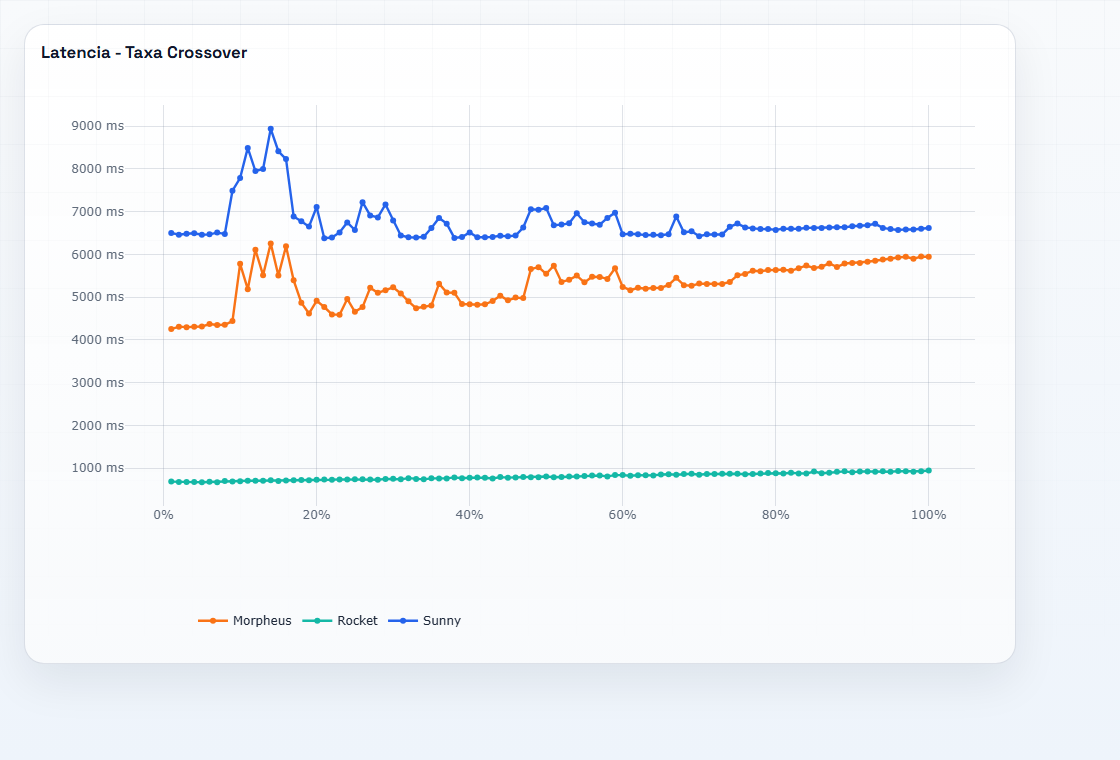
\includegraphics[width=0.9\linewidth,keepaspectratio]{figuras/benchmark/Figura_51_dashboard_latencia_i3_taxa_crossover.png}
\fonteautores
\end{figure}

\begin{figure}[H]
\centering
\caption{Latência média na variação da taxa de crossover no Cenário i5/full, conforme visualização filtrada no Dashboard IGRIS}
\label{fig:benchmark-latencia-crossover-i5}
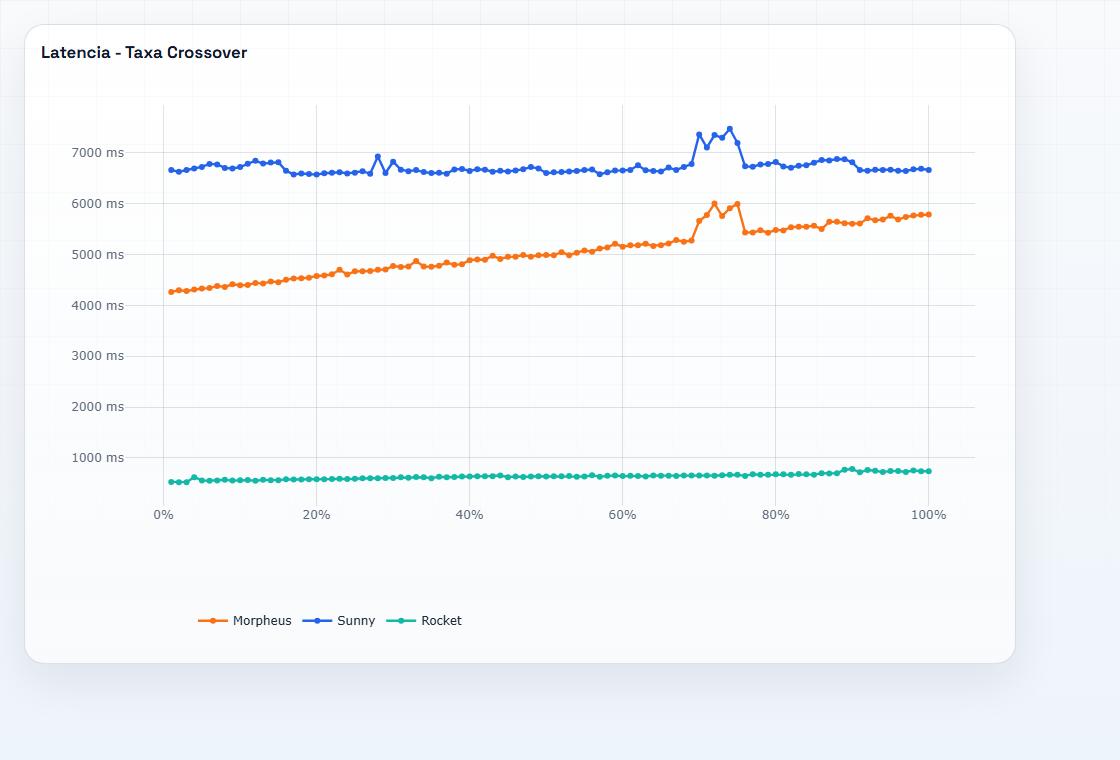
\includegraphics[width=0.9\linewidth,keepaspectratio]{figuras/benchmark/Figura_52_dashboard_latencia_i5_taxa_crossover.png}
\fonteautores
\end{figure}

Em parâmetros como tamanho da população, número de gerações, taxa de elitismo, pontuação base, penalidade de conflito, bônus de diversidade e tamanho do torneio, o Morpheus também apresentou médias de tempo inferiores às do Sunny. Esse comportamento reforça que sua vantagem não ocorreu apenas em um recorte específico, mas apareceu em diferentes dimensões do benchmark.

A principal exceção observada na comparação entre Morpheus e Sunny foi a taxa de mutação. Nesse parâmetro, o Sunny apresentou tempo médio menor nos dois cenários. No cenário i3, sua vantagem foi de aproximadamente 9,50\%. No cenário i5/full, a vantagem foi de aproximadamente 6,19\%. Esse resultado mostra que o Sunny pode apresentar desempenho competitivo em configurações específicas, mesmo não superando o Morpheus no agregado global.

\begin{figure}[H]
\centering
\caption{Latência média na variação da taxa de mutação no Cenário i3, conforme visualização filtrada no Dashboard IGRIS}
\label{fig:benchmark-latencia-mutacao-i3}
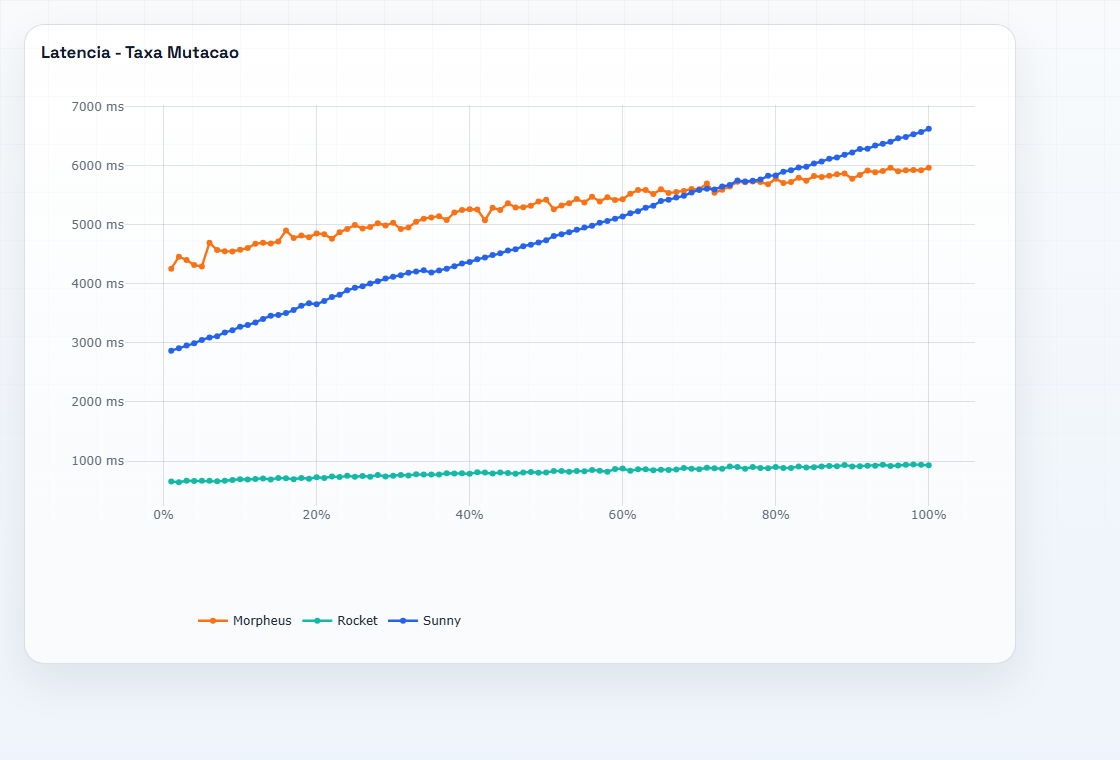
\includegraphics[width=0.9\linewidth,keepaspectratio]{figuras/benchmark/Figura_53_dashboard_latencia_i3_taxa_mutacao.png}
\fonteautores
\end{figure}

\begin{figure}[H]
\centering
\caption{Latência média na variação da taxa de mutação no Cenário i5/full, conforme visualização filtrada no Dashboard IGRIS}
\label{fig:benchmark-latencia-mutacao-i5}
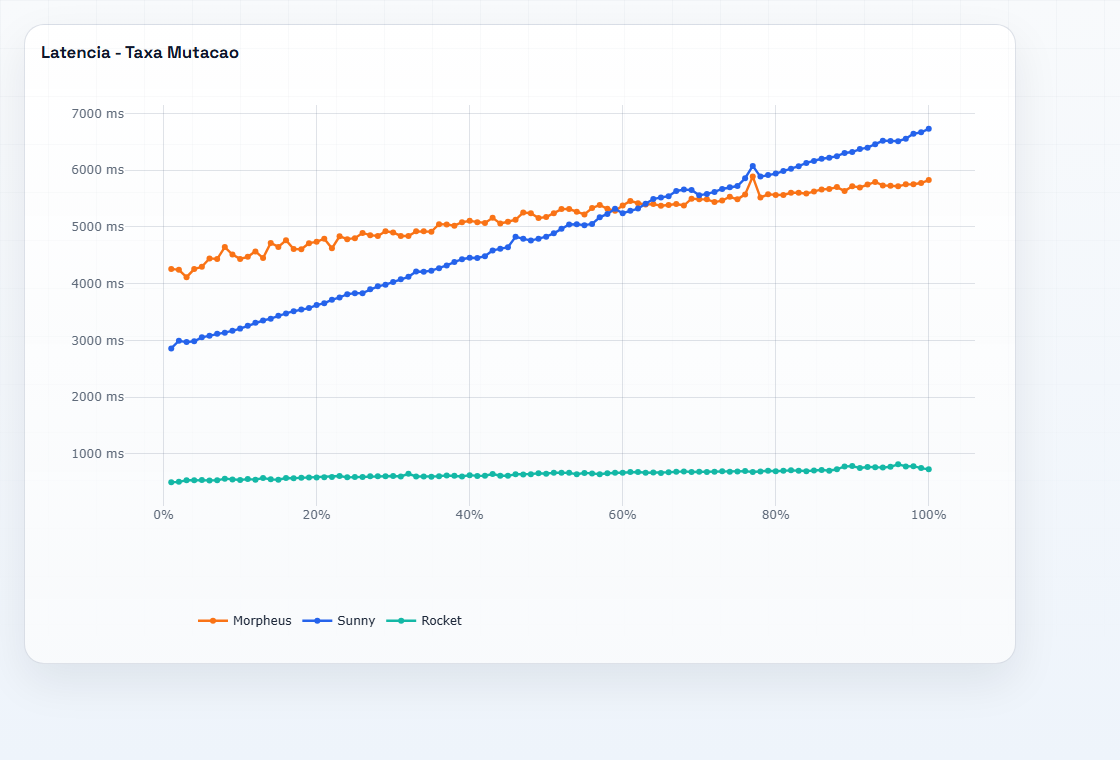
\includegraphics[width=0.9\linewidth,keepaspectratio]{figuras/benchmark/Figura_54_dashboard_latencia_i5_taxa_mutacao.png}
\fonteautores
\end{figure}

A incorporação do Rocket amplia essa leitura. No cenário i3, as maiores médias do Rocket ocorreram em taxa de elitismo, com 946,65 ms, tamanho do torneio, com 946,01 ms, penalidade de conflito, com 924,98 ms, bônus de diversidade, com 922,08 ms, e pontuação base, com 913,11 ms. No cenário i5/full, as maiores médias ocorreram em taxa de elitismo, com 738,94 ms, tamanho do torneio, com 734,23 ms, bônus de diversidade, com 732,38 ms, pontuação base, com 727,94 ms, e penalidade de conflito, com 727,61 ms.

Mesmo nos parâmetros mais custosos para o Rocket, suas médias permaneceram inferiores às médias observadas para Morpheus e Sunny nos mesmos cenários. No i3, por exemplo, os parâmetros menos custosos para Morpheus ficaram acima de 3.000 ms, enquanto o Rocket permaneceu abaixo de 1.000 ms em todos os agrupamentos paramétricos. No i5/full, o comportamento foi semelhante, com o Rocket abaixo de 740 ms nos agrupamentos de maior latência média e os demais algoritmos em patamares superiores.

Essa diferença pode indicar que o custo das operações evolutivas do Rocket foi reduzido pela combinação de estruturas indexadas, população e \textit{fitness} avaliados de forma concorrente e reparo local restrito a candidatos já filtrados. Entretanto, os dados não isolam o efeito de cada componente arquitetural. Portanto, não é possível afirmar se a vantagem decorre principalmente da linguagem, do modelo de concorrência, das estruturas de dados, da implementação do reparo ou da combinação desses fatores.

A análise por parâmetro deve ser interpretada com cautela, pois os resultados representam agrupamentos experimentais do benchmark progressivo. Portanto, não se trata necessariamente de um experimento isolado em que apenas uma variável foi alterada sob controle absoluto. Ainda assim, os dados permitem identificar em quais dimensões paramétricas as diferenças entre os algoritmos se tornaram mais evidentes.

De modo geral, o Rocket apresentou o menor tempo médio ao longo dos parâmetros avaliados, o Morpheus apresentou maior consistência operacional que o Sunny na maioria dos parâmetros, e o Sunny demonstrou vantagem pontual sobre o Morpheus na taxa de mutação. Dessa forma, a análise paramétrica confirma a tendência observada nos resultados gerais e mostra que a inclusão do Rocket revela um nível adicional de eficiência que não era observável na comparação apenas entre Morpheus e Sunny.
